\documentclass[conference,onecolumn, catalan]{IEEEtran}
\IEEEoverridecommandlockouts
% The preceding line is only needed to identify funding in the first footnote. If that is unneeded, please comment it out.
\usepackage{comment}
\usepackage{hyperref}
\usepackage{cite}
\usepackage{amsmath,amssymb,amsfonts}
\usepackage{algorithmic}
\usepackage{textcomp}
\usepackage{xcolor}
\def\BibTeX{{\rm B\kern-.05em{\sc i\kern-.025em b}\kern-.08em
    T\kern-.1667em\lower.7ex\hbox{E}\kern-.125emX}}
\newtheorem{theorem}{Teorema}
\usepackage{listings}
\usepackage{babel}
\usepackage{geometry}% http://ctan.org/pkg/geometry
\usepackage{graphicx}% http://ctan.org/pkg/graphicx
\usepackage{color} %red, green, blue, yellow, cyan, magenta, black, white
\definecolor{mygreen}{RGB}{28,172,0} % color values Red, Green, Blue
\definecolor{mylilas}{RGB}{170,55,241}
\lstset{language=Matlab,%
    %basicstyle=\color{red},
    breaklines=true,%
    morekeywords={matlab2tikz},
    keywordstyle=\color{blue},%
    morekeywords=[2]{1}, keywordstyle=[2]{\color{black}},
    identifierstyle=\color{black},%
    stringstyle=\color{mylilas},
    commentstyle=\color{mygreen},%
    showstringspaces=false,%without this there will be a symbol in the places where there is a space
    numbers=left,%
    basicstyle=\small,
    numbers = none,
    %numberstyle=none,% size of the numbers
    %numbersep=2pt, % this defines how far the numbers are from the text
    emph=[1]{for,end,break},emphstyle=[1]\color{red}, %some words to emphasise
    %emph=[2]{word1,word2}, emphstyle=[2]{style},    
}

\newenvironment{changemargin}[2]{%
\begin{list}{}{%
\setlength{\topsep}{0pt}%
\setlength{\leftmargin}{#1}%
\setlength{\rightmargin}{#2}%
\setlength{\listparindent}{\parindent}%
\setlength{\itemindent}{\parindent}%
\setlength{\parsep}{\parskip}%
}%
\item[]}{\end{list}}

\title{Segon Informe de Progrés del TFG: \\ \vspace{0.2cm} {\huge \textit{ Desenvolupament d'un ``core" didàctic de RISC-V\ }} }
\author{
\IEEEauthorblockN{Pau Casacuberta Orta}
\IEEEauthorblockA{
\textit{Autonomous University of Barcelona}\\
Cerdanyola del Vallès, Barcelona 08193\\
pau.casacubertao@e-campus.uab.cat\\}}

\usepackage[owncaptions, tablegrid]{vhistory}
\renewcommand{\vhhistoryname}{Històric de versions}
\renewcommand{\vhversionname}{Versió}
\renewcommand{\vhdatename}{Data}
\renewcommand{\vhauthorname}{Autor(s)}
\renewcommand{\vhchangename}{Descripció}
\newcommand\todo[1]{\textcolor{red}{#1}}

\begin{document}

\maketitle

\begin{versionhistory}
    \vhEntry{0.1}{07.11.19}{Pau}{Creació del primer esborrany.}
    \vhEntry{1.0}{10.11.19}{Pau}{Modificacions proposades pel tutor (Lluís), afegir documentació CSR i accés a memòria i Gantt simple.}
\end{versionhistory}


\begin{abstract}
La finalitat d'aquest document és el de consignar els avenços efectuats en el desenvolupament del treball.
\end{abstract}

\section{Seguiment}

A data de 7 de novembre de 2019 s'ha consolidat part de les tasques per al desenvolupament del projecte. 
Les tasques de recerca inicial, i la majoria de les de programació s'han dut a terme. 

El resultat es pot veure a GitHub\cite{casacuberta_orta_4a1c0/rv32i-verilog_2019}.En concret com s'han implementat els blocs necessaris per a que el core pugui executar tot el repertori RV32I (a excepció de les crides \textit{FENCE} ja que no es faran servir en aquesta implementació). 
També s'han implementat els tests corresponents per a verificar el correcte funcionament al executar instruccions.

Durant aquest període s'han produït reunions amb en Raimon i una amb la resta del grup per presentar el codi. D'aquesta última va sorgir la necessitat d'implementar els registres de control i d'estat (CSR) i modificar l'accés a la memòria de dades per a poder determinar a través d'una màscara quins bytes d'una paraula de memòria s'han d'escriure.

La implementació dels mòduls bàsics d'un processador general (unitat de control, unitat d'execució, banc de registres i comptador de programa) no han sigut massa complicades degut a que a la bibliografia \cite{patterson_computer_2018} queda ben explicada. En canvi la implementació dels registres de control i d'estat (CSR) ha suposat un esforç major degut a que no hi ha exemples d'implementació, a part d'alguns comentaris al document de l'especificació del ISA \cite{waterman_volume_2019}. Per aquest motiu s'han consultat altres fonts com \cite{noauthor_fe310g:_2017} i \cite{noauthor_control_nodate}.

A l'hora de determinar els senyals i la lògica per a la nova memòria de dades basant-se en una implementació del projecte picorv32 \cite{wolf_cliffordwolf/picorv32_2019}. Aquesta implementació permet guardar dades de 8, 16 o 32 bits en un sol accés afegint un senyal de control extra.

Al desenvolupar les tasques anteriorment esmentades s'ha notat que fan falta ajustar el nombre d'hores de dedicació a diferents apartats, en concret la part d'implementació rep un increment d'hores.

\begin{figure}[!ht]
\centering
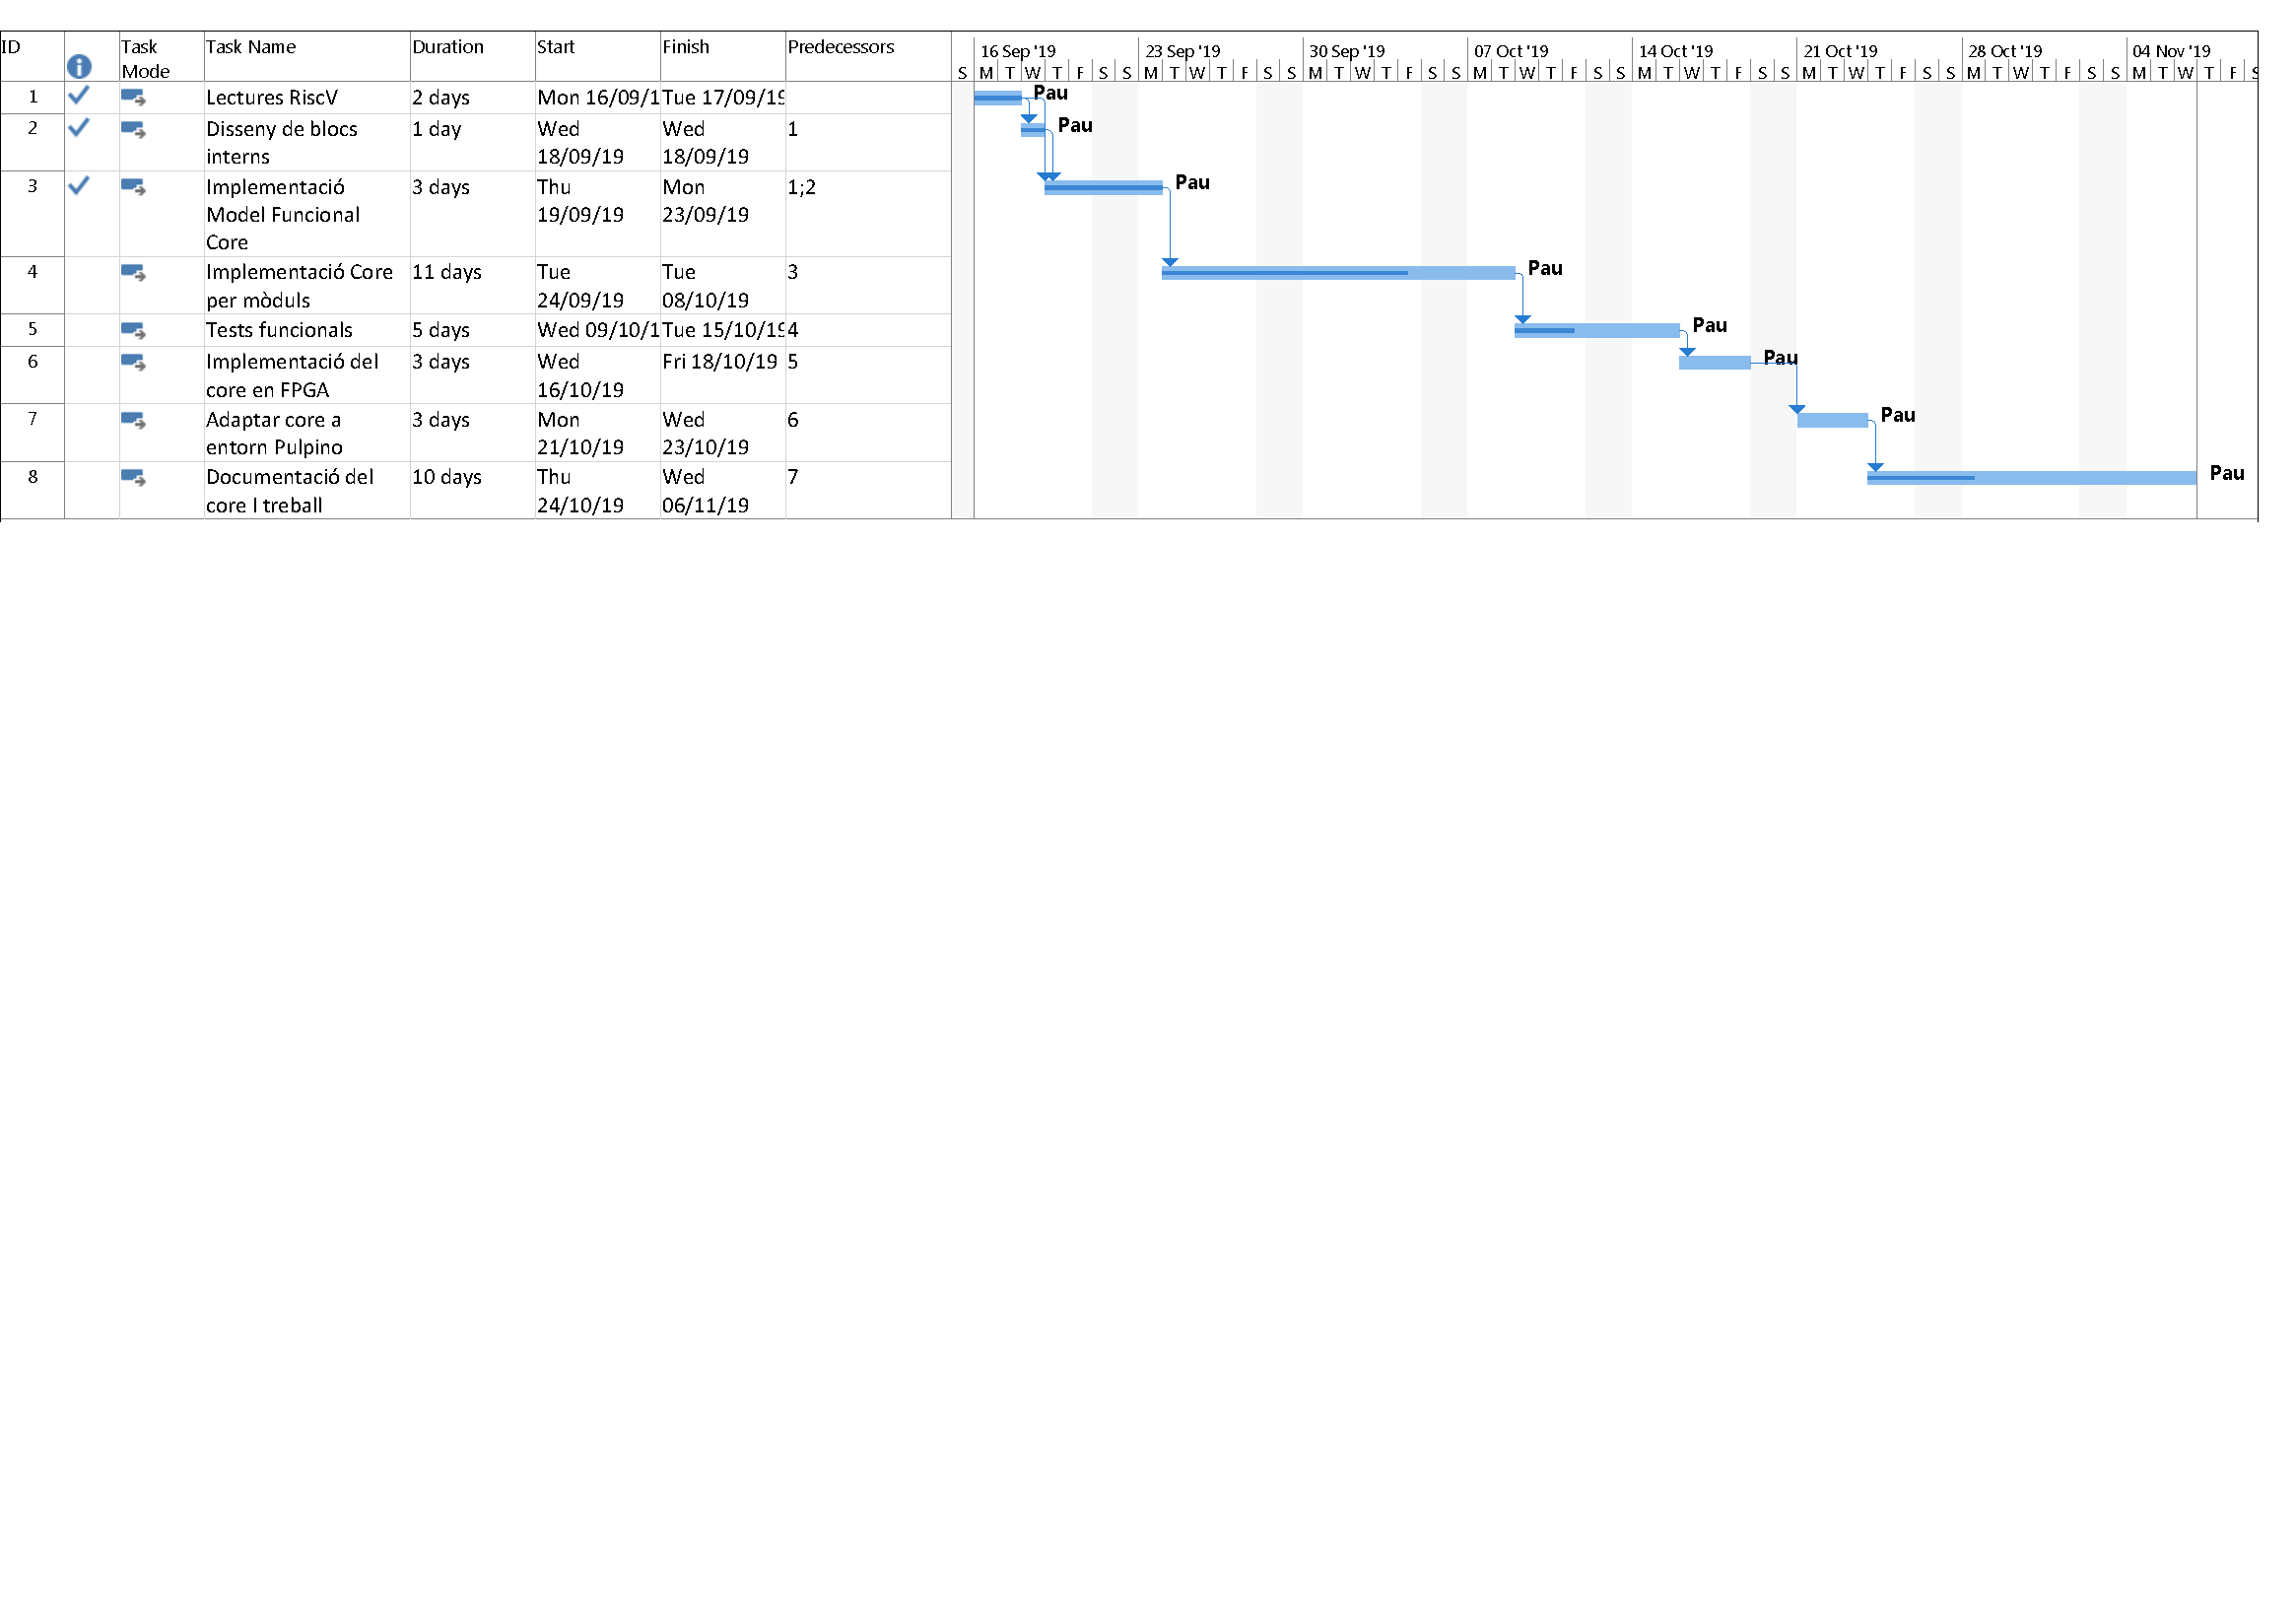
\includegraphics[width=\textwidth]{gantt.pdf}
\caption{Gantt bàsic amb la planificació a falta de subdividir en tasques.}
\label{fig:gantt}
\end{figure}

\section{Canvis}

Veient el ritme en desenvolupament del projecte, i per reduir riscos per la seva finalització, s'ha decidit eliminar dels objectius la implementació del core amb pipeline degut a que aquesta pot comportar un temps elevat per a ésser completada en el calendari establert.

En el següent informe es detallarà més el diagrama de Gantt (figura \ref{fig:gantt}) (incloent més tasques).




\section{Metodologia}

En relació a la metodologia per a desenvolupar les tasques es la mateixa que es determina en l'informe inicial. Bisetmanalment es planifica una reunió amb el tutor (ja sigui personalment o via correu electrònic) per comentar els avenços i planificar les següents tasques que es desenvoluparan fins a la següent reunió. Proposo utitilitzar l'eina de gestió de projectes que proporciona GitHub la qual funciona com una taulell kanban (Permet gestionar tasques entre diferents columnes, ToDo, InProgress i Done) \cite{noauthor_4a1c0/rv32i-verilog_nodate}. 

En relació a edició d'informes es proposa fer un repositori de git per a cada document per a poder fer un seguiment de versions i poder accedir a cada versió de manera oberta.






\bibliographystyle{IEEEtran}
\bibliography{references.bib}


\end{document}
